\chapter{Acoplamiento de modos P}
En electrodinámica, es posible asociar las interacciones dipolares eléctricas con los polinomios de Legendre de orden 2, $P_2(\cos(\theta))$, con $\theta$ el ángulo que forman los dipolos entre sí. Se suele llamar \textit{ángulo mágico} al ángulo $\theta_m \approx 54.7^\circ$, pues anula el término de interacción dipolar [ref]. 

Este capítulo tiene como protagonistas a los llamados modos P o modos dipolares verticales, cuya excitación es posible al superar la condición de corte (longitud de onda lo suficiemente pequeña y tanto contraste $\Delta n$ como ancho de la guía lo suficientemente grandes). 



\section{Acopladores}
Al considerar qué sucede con el acoplamiento entre modos $p_y$ de guías elípticas, se pueden distinguir dos casos límite: 1) Para acopladores horizontales, el acoplamiento $C_\pi$ tiene signo positivo. 2) Para acopladores verticales, el acoplamiento $C_\sigma$ tiene signo negativo. Esta fenomenología es análoga a la que sucede en los enlaces químicos $\sigma$ y $\pi$ de las cadenas de carbono orgánicas. 
\begin{figure}[H]
	\centering
	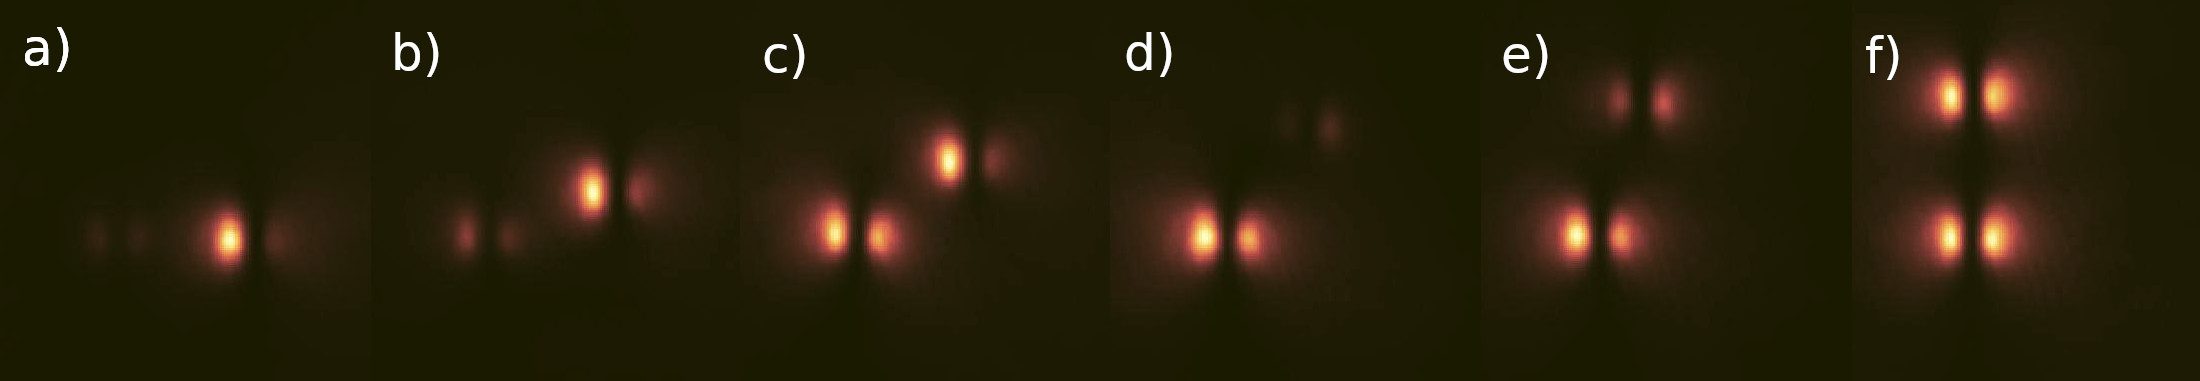
\includegraphics[width=\linewidth]{media/dipoles}
	\caption{Barrido en ángulo que captura el paso por acoplamiento nulo.}
\end{figure}
\section{Redes tipo panal de abeja}

